% Options for packages loaded elsewhere
\PassOptionsToPackage{unicode}{hyperref}
\PassOptionsToPackage{hyphens}{url}
%
\documentclass[
  english,
  man]{apa6}
\usepackage{lmodern}
\usepackage{amssymb,amsmath}
\usepackage{ifxetex,ifluatex}
\ifnum 0\ifxetex 1\fi\ifluatex 1\fi=0 % if pdftex
  \usepackage[T1]{fontenc}
  \usepackage[utf8]{inputenc}
  \usepackage{textcomp} % provide euro and other symbols
\else % if luatex or xetex
  \usepackage{unicode-math}
  \defaultfontfeatures{Scale=MatchLowercase}
  \defaultfontfeatures[\rmfamily]{Ligatures=TeX,Scale=1}
\fi
% Use upquote if available, for straight quotes in verbatim environments
\IfFileExists{upquote.sty}{\usepackage{upquote}}{}
\IfFileExists{microtype.sty}{% use microtype if available
  \usepackage[]{microtype}
  \UseMicrotypeSet[protrusion]{basicmath} % disable protrusion for tt fonts
}{}
\makeatletter
\@ifundefined{KOMAClassName}{% if non-KOMA class
  \IfFileExists{parskip.sty}{%
    \usepackage{parskip}
  }{% else
    \setlength{\parindent}{0pt}
    \setlength{\parskip}{6pt plus 2pt minus 1pt}}
}{% if KOMA class
  \KOMAoptions{parskip=half}}
\makeatother
\usepackage{xcolor}
\IfFileExists{xurl.sty}{\usepackage{xurl}}{} % add URL line breaks if available
\IfFileExists{bookmark.sty}{\usepackage{bookmark}}{\usepackage{hyperref}}
\hypersetup{
  pdftitle={Going from coarse landings data to fine scale species distribution},
  pdfauthor={Author11 \& Author21,2},
  pdfkeywords={keywords},
  hidelinks,
  pdfcreator={LaTeX via pandoc}}
\urlstyle{same} % disable monospaced font for URLs
\usepackage{graphicx,grffile}
\makeatletter
\def\maxwidth{\ifdim\Gin@nat@width>\linewidth\linewidth\else\Gin@nat@width\fi}
\def\maxheight{\ifdim\Gin@nat@height>\textheight\textheight\else\Gin@nat@height\fi}
\makeatother
% Scale images if necessary, so that they will not overflow the page
% margins by default, and it is still possible to overwrite the defaults
% using explicit options in \includegraphics[width, height, ...]{}
\setkeys{Gin}{width=\maxwidth,height=\maxheight,keepaspectratio}
% Set default figure placement to htbp
\makeatletter
\def\fps@figure{htbp}
\makeatother
\setlength{\emergencystretch}{3em} % prevent overfull lines
\providecommand{\tightlist}{%
  \setlength{\itemsep}{0pt}\setlength{\parskip}{0pt}}
\setcounter{secnumdepth}{-\maxdimen} % remove section numbering
% Make \paragraph and \subparagraph free-standing
\ifx\paragraph\undefined\else
  \let\oldparagraph\paragraph
  \renewcommand{\paragraph}[1]{\oldparagraph{#1}\mbox{}}
\fi
\ifx\subparagraph\undefined\else
  \let\oldsubparagraph\subparagraph
  \renewcommand{\subparagraph}[1]{\oldsubparagraph{#1}\mbox{}}
\fi
% Manuscript styling
\usepackage{upgreek}
\captionsetup{font=singlespacing,justification=justified}

% Table formatting
\usepackage{longtable}
\usepackage{lscape}
% \usepackage[counterclockwise]{rotating}   % Landscape page setup for large tables
\usepackage{multirow}		% Table styling
\usepackage{tabularx}		% Control Column width
\usepackage[flushleft]{threeparttable}	% Allows for three part tables with a specified notes section
\usepackage{threeparttablex}            % Lets threeparttable work with longtable

% Create new environments so endfloat can handle them
% \newenvironment{ltable}
%   {\begin{landscape}\centering\begin{threeparttable}}
%   {\end{threeparttable}\end{landscape}}
\newenvironment{lltable}{\begin{landscape}\centering\begin{ThreePartTable}}{\end{ThreePartTable}\end{landscape}}

% Enables adjusting longtable caption width to table width
% Solution found at http://golatex.de/longtable-mit-caption-so-breit-wie-die-tabelle-t15767.html
\makeatletter
\newcommand\LastLTentrywidth{1em}
\newlength\longtablewidth
\setlength{\longtablewidth}{1in}
\newcommand{\getlongtablewidth}{\begingroup \ifcsname LT@\roman{LT@tables}\endcsname \global\longtablewidth=0pt \renewcommand{\LT@entry}[2]{\global\advance\longtablewidth by ##2\relax\gdef\LastLTentrywidth{##2}}\@nameuse{LT@\roman{LT@tables}} \fi \endgroup}

% \setlength{\parindent}{0.5in}
% \setlength{\parskip}{0pt plus 0pt minus 0pt}

% \usepackage{etoolbox}
\makeatletter
\patchcmd{\HyOrg@maketitle}
  {\section{\normalfont\normalsize\abstractname}}
  {\section*{\normalfont\normalsize\abstractname}}
  {}{\typeout{Failed to patch abstract.}}
\patchcmd{\HyOrg@maketitle}
  {\section{\protect\normalfont{\@title}}}
  {\section*{\protect\normalfont{\@title}}}
  {}{\typeout{Failed to patch title.}}
\makeatother
\shorttitle{SHORTTITLE}
\keywords{keywords\newline\indent Word count: X}
\DeclareDelayedFloatFlavor{ThreePartTable}{table}
\DeclareDelayedFloatFlavor{lltable}{table}
\DeclareDelayedFloatFlavor*{longtable}{table}
\makeatletter
\renewcommand{\efloat@iwrite}[1]{\immediate\expandafter\protected@write\csname efloat@post#1\endcsname{}}
\makeatother
\usepackage{lineno}

\linenumbers
\usepackage{csquotes}
\usepackage{graphicx}
\usepackage{caption}
\ifxetex
  % Load polyglossia as late as possible: uses bidi with RTL langages (e.g. Hebrew, Arabic)
  \usepackage{polyglossia}
  \setmainlanguage[]{english}
\else
  \usepackage[shorthands=off,main=english]{babel}
\fi

\title{Going from coarse landings data to fine scale species distribution}
\author{Author1\textsuperscript{1} \& Author2\textsuperscript{1,2}}
\date{}


\authornote{

Test

The authors made the following contributions. Author1: Conceptualization, Writing - Original Draft Preparation, Writing - Review \& Editing; Author2: Writing - Review \& Editing.

Correspondence concerning this article should be addressed to Author1, Postal address. E-mail: \href{mailto:my@email.com}{\nolinkurl{my@email.com}}

}

\affiliation{\vspace{0.5cm}\textsuperscript{1} Instit1\\\textsuperscript{2} Instit2}

\abstract{
Test
}



\begin{document}
\maketitle

References for change of support issues in integrated modelling:

\url{https://esajournals.onlinelibrary.wiley.com/doi/epdf/10.1002/ecy.2710}

\url{https://besjournals.onlinelibrary.wiley.com/doi/full/10.1111/2041-210X.12793}

\url{https://www.sciencedirect.com/science/article/pii/S0169534719302551\#b0010}

\url{https://www.sciencedirect.com/science/article/pii/S0006320721001993}

\hypertarget{material-and-methods}{%
\section{Material and methods}\label{material-and-methods}}

We base our approach on the model developped by Alglave et al. (2022). In this framework, all observations were supposed to be realised at the same scale.

Here, we extend the framework to potentially provide fine scale predictions from data that have a coarse resolution (landings data) and combine these data with other (more accurate) datasets such as scientific data.

In the following we describe the processes from a modeling perspective in order to clearly define the problem we adress.

\hypertarget{defining-the-problem-from-a-modelling-point-of-view}{%
\subsection{Defining the problem from a modelling point of view}\label{defining-the-problem-from-a-modelling-point-of-view}}

\textbf{Definition of the variables}

Let's define the latent field \(S\) and the punctual observations \(Y\). \(S\) is a spatial log-Gaussian Field (GF) defined as \(\log(S(x))=\mu+\beta . \Gamma(x) + \delta(x)\) (Figure \label{fig:ParBiasSingle}). We consider a discrete study domain where \(x \in [\![1,n]\!]\) stands for the discrete locations. \(\beta . \Gamma(x)\) is the covariate term with \(\Gamma\) the matrix of design of the covariates and \(\beta\) the effect of the covariates. \(\delta(x)\) is a GF capturing spatial correlation (\(\delta \sim \mathcal{N}(0,\Sigma)\)).

All fishing locations \(x_i\) are supposed to be known through VMS data. At each fishing location \(x_i\), fishermen realize a catch \(Y_i\) conditionnally on the latent field values. Observations are supposed to follow some distribution \(\mathcal{L}_Y\). In our case, data are zero-inflated positive continuous data and so they are modelled through a zero-inflated lognormal model previously introduced by Thorson (2018) and already used in Alglave et al. (2022).

\[Y_i | S(x_i), x_i \sim \mathcal{L}_Y(S(x_i),\xi,\sigma)\]

\(\mathcal{L}_Y\) is decomposed it 2 parts:

\begin{itemize}
\item
  the probability to obtain a zero-catch which is modelled as Bernoulli variable with probability \(p_{i}=\exp(-e^\xi .S(x_{i}))\).
\item
  if the catch is positive, the probability to obtain some value \(y_i\) is modelled through a continous distribution \(\operatorname{L}\) (here a lognormal distribution - its parameterization is described in SM\ldots)) with mean component \(\frac{S(x_{i})}{1-p_{i}}\) and variance term \(\sigma^2\).
\end{itemize}

\[
\operatorname{P}\left(Y_i=y_{i} | x_i, S(x_i)\right) =
\left\{
    \begin{array}{ll}
        p_i & \text { if } y_{i}=0 \\
        \left(1-p_i\right) \cdot \operatorname{L}\left(y_{i },\frac{S(x_i)}{\left(1 - p_i\right)},\sigma^{2} \right) & \text { if } y_{i} > 0
    \end{array}
\right.
\]

Fishermen must declare what they catch at the level of the statistical rectangle. The declaration \(D_j\) is then a summation of all the \(Y_i\) realized on the fishing positions belonging to the catch declaration \(D_j\) (\(j\) is the declaration index). We denote the vector of the fishing observations belonging to declaration \(D_j\) as \(\mathcal{P}_j\). Then, \(D_j\) can be expressed as:

\[D_j=\sum_{i \in \mathcal{P}_j}{Y_{i}}\]

The punctual observations \(Y_i\) are indexed through \(i \in [\![1,m_j]\!]\) with \(m_j\) the number of fishing positions belonging to the \(j^{th}\) declaration. \(D_j\) are commonly recorded in logbooks data.

\textbf{Catch reallocation: uniform reallocation or model-based reallocation}

\(D_j\) are known through logbooks data, \(x_i\) are known through VMS data. Consequently, in standard processing \(D_j\) are reallocated uniformly on related \(x_i\) so that derived punctual observations \(Y^*_i\) are computed as \(Y^*_i=D_j/m_j\). This is what we call uniform (or proportional) reallocation. In this case, inference of species distribution is directly computed through reallocated \(Y^*_i\) assuming these are the exact punctual observations. This strongly simplifies the actual process of observation and have most likely repercussion on model performance.

To overcome such limitation, an alternative is to consider that only the catch declarations \(D_j\) are observed while \(Y_i\) are not (they are latent variables).

Such way, we define some distribution \(\mathcal{L}_D\) as the distribution of the catch declarations:

\[D_j | S_{\mathcal{P}_j},\mathcal{P}_j \sim \mathcal{L}_D( S_{\mathcal{P}_j},\xi,\sigma)\]

with \(S_{\mathcal{P}_j}=(S(x_1),...,S(x_i), ...,S(x_{m_j}))\). As \(D_j=\sum_{i \in \mathcal{P}_j}{Y_{i}}\), it is possible to relate \(D_j\), \(Y_i\) and \(S_{\mathcal{P}_j}\) through the distribution \(\mathcal{L}_Y\) and \(\mathcal{L}_D\). Our approach is to match the moments of \(D_j\) (obtained from the moments of \(\mathcal{L}_Y\) i.e.~the probability distribution of \(Y\)) and \(\mathcal{L}_D\) and then to infer \(S(x)\) and \(Y_i\) from \(D_j\). This is what we call model-based reallocation. The models based on declaration \(D_j\) will be referred as the declaration-based models.

In the following, \(Y\) and \(D\) will be assumed conditionnal over the fishing positions and the latent field values, but for notation simplicity they will be simply denoted as \(Y_i\) or \(D_j\) instead of \(Y_i \vert x_i, S(x_i)\) and \(D_j | S_{\mathcal{P}_j},\mathcal{P}_j\).

\textbf{Matching \(\mathcal{L}_Y\) and \(\mathcal{L}_D\)}

First, as at the \(Y\) level, the declarations can be decomposed in 2 components: (1) the probability to obtain a zero value declaration and, if the declaration is positive, (2) the probability to obtain some declaration value \(d_j\).

\begin{enumerate}
\def\labelenumi{(\arabic{enumi})}
\tightlist
\item
  We derive the probability to obtain a zero-declaration \(P(D_j = 0)\) by simply multiplying the probability to obtain a zero-punctual observation \(P(Y_i=0 )\) to all fishing points \(x_i \in \mathcal{P}_j\).
\end{enumerate}

\begin{align*}
P(D_j = 0) & = \prod_{i\in \mathcal{P}_j} P(Y_{i} = 0),\nonumber \\
                      & = \exp{ \left \lbrace- \sum_{i\in \mathcal{P}_j} e^{\xi}. S(x_{i})\right \rbrace} = \pi_j.
\end{align*}

\begin{enumerate}
\def\labelenumi{(\arabic{enumi})}
\setcounter{enumi}{1}
\tightlist
\item
  If the declaration is positive, we assume the probability to obtain catch \(d_j\) follows a continous distribution \(\mathcal{L}_{D_j|D_j>0}\) with mean component \(\mu_j\) and variance component \(\sigma_j\). These are expressed as a function of the two first moments of \(\mathcal{L}_Y\). In other words, from \(\mathcal{L}_Y\) we can derive \(E(D_j \vert D_j > 0)\) and \(Var(D_j \vert D_j > 0)\). If we consider \(\mathcal{L}_{D_j|D_j>0}\) is lognormal (with parameterization described in SM \ldots) then, \(\mu_j = E(D|D_j>0)\) and \(\sigma_j = ln(\frac{Var(D|D_j>0)}{E(D|D_j>0)^2} + 1)\).
\end{enumerate}

The expressions of \(E(D_j \vert D_j > 0)\) and \(Var(D_j \vert D_j > 0)\) are given by:

\[E(D_j \vert D_j > 0)=\frac{\sum_{i \in \mathcal{P}_j} S(x_{i})}{1-\pi_j}\]
\[Var(D_j \vert D_j > 0) = \frac{\sum_{i \in \mathcal{P}_j} Var(Y_{i})}{1-\pi_j} - \frac{\pi_j}{(1-\pi_j)^2}E(D_j)^2\]
\[Var(Y_{i})=\frac{S(x_{i})^2}{1-p_{i}}(e^{\sigma^2}-(1-p_{i}))\]

All calculations to obtain these formulas are available in SM. By linking \(\mathcal{L}_Y\) and \(\mathcal{L}_D\), we intend to better follow the observation process of the commercial data and potentially improve inference compared with the approximation realized through uniform reallocation.

The inference procedure is realized through Template Model Builder (TMB), an effective tool to build hierarchical models and perform maximum likelihood estimation through automatic differentiation and Laplace Approximation (Kristensen, Nielsen, Berg, Skaug, \& Bell, 2016).

\begin{figure}
\centering
\includegraphics{images/realloc.png}
\caption{\label{fig:ParBiasSingle} Reallocation process.}
\end{figure}

\hypertarget{simulation-estimation}{%
\subsection{Simulation-estimation}\label{simulation-estimation}}

To evaluate what bring the performance of the new approach, we assess model performance through simulation-estimation.

First, we limit the study to simaultions over a single square. Only commercial data feed the model and the expression of the latent field in both simulation and estimation is simplified (the variability only depends on one covariate, not on a spatial random term) in order to explore the base properties of the model.

Then, we extend the simulation-estimation study to several rectangles to get closer to a real case study configuration. We add a spatial random effect in the latent field (for both simulation and estimation) and, in addition to commercial data, we also simulate scientific data to explore the contribution of both datasets in inference.

In these two steps, the covariate is modelled as a continous GRF that we suppose known at each point of the grid. The covariate effect is fixed to \(\beta_S=2\) and the intercept is also fixed to \(\mu=2\). The random effect (for the several rectangle simulation) is modelled as a Matérn GRF, but is supposed unkwnon over the area. Regarding commercial data, to fit the real data the number of fishing pings per declaration is fixed to 10 as it is the average number of fishing locations for one declaration. All parameterizations are detailed in the table \ldots{} .

Each time we compare several model configurations and evaluate these in regards to 2 metrics:

\begin{itemize}
\tightlist
\item
  the MSPE which quantifies the accuracy of the spatial predictions of the latent field over the spatial domain.
\end{itemize}

\[MSPE=\frac{\sum_x (S(x) - \hat{S}(x) ) ^2}{n}\]

\begin{itemize}
\tightlist
\item
  the parameter of the species habitat relationship \(\beta_S\) compared with its estimate \(\hat \beta_S\).
\end{itemize}

\textbf{Single-square simulations}

Two important variables may affect the accuracy of model outputs.

First, the amount of commercial data; it is expected that when increasing the amount of data the accuracy of the predictions will be improved. In simulations, we progressively increase the number of fishing positions (10, 100 and 1000 fishing pings). As there are 10 pings per declaration, this means that the number of declarations increases respectively (1, 10 and 100 declarations).

Furthermore, the samples belonging to a single declaration can be sampled in a single restricted zone or can mix catches from distinct zones (within a unique statistical rectangle). Note that we make a distinction between fishing zones and statistical rectangles, fishing zones are included in a statistical rectangle and there can be several fishing zones within a statistical rectangles. In other words, a declaration can mix catches that have been realized in zones of high biomass and in zones of low biomass. For instance, a declaration can aggregate data from several fishing operations that occured the same day within the same statistical rectangle, but that were realized on 2 distinct types of fishing grounds (and then on two distinct habitats). Reallocating uniformly the declaration will strongly homogeneise the actual catch, will mix up information from to different locations and then may lead to a strong loss of accuracy in model outputs. It is expected that when the number of fishing zones within a declaration increases, the accuracy of the model outputs decreases. To assess this effect of such process, we simulated the pings of a fishing declaration assuming they were either realized in a single zone, in 3 distinct zones or in 5 distinct zones.

Concretely, for each fishing declaration the fishing pings are sampled in 2 steps: first the centroid of the zones are randomly sampled over the statistical rectangle (here the simulation domain) and then the fishing positions are sampled within the radius of the centroid of the zones. The zone size was chosen to be a square of side 7. This is a realistic order of magnitude if we consider each zone is one fishing operation and that for each fishing operation the distance of the operation will not exceed 30km.

At each fishing position a catch is realized conditionnally on the value of the latent field at the related positions and follow the probability distribution described above (\(\mathcal{L}_y\)).

We compare three simulation/estimation configurations:

\begin{itemize}
\item
  a golden standard configuration: observations are known exactly and the standard model is fitted to the data.
\item
  a configuration corresponding to the actual situation (uniform reallocation): simulated catch are reallocated over fishing locations, the standard model is fitted to the data (i.e.~the one working at the level of \(Y_i^*\)).
\item
  a configuration corresponding to our alternative approach: simulated catch are reallocated over fishing locations, the alternative model is fitted to the data (i.e.~the one working at the level of \(D_j\)).
\end{itemize}

In addition to the metrics we introduced to compare model configuration (\(MSPE\) and species-habitat parameter \(\beta_S\)), we also assess the simulated/estimated values for the intercept \(\mu\), the observation variance parameter \(\sigma^2\) and the zero-inflation parameter \(\xi\).

\hypertarget{multiple-squares-simulations}{%
\subsubsection{Multiple-squares simulations}\label{multiple-squares-simulations}}

In this case, we extend the study to more than one single rectangle, we simulate scientific data and include these in inference. Finally, in addition to the covariate, we also simulate/estimate a spatial random effect in the latent field.

The study area is based on the case study; it includes the whole coast of the Bay of Biscay (Figure \ref{fig:MapSeveral}A). To tailor the case study, we simulate 3000 of fishing positions regrouped in 300 declarations (10 pings per declaration). Commercial data may not cover the full area, and consequently we allow the commercial samples to cover only 2/3 ot the area. Similarly to the single-square simulations, the sampling of the commercial points of a declaration is realized in 3 steps. (1) The declarations is affected to one of the ICES rectangle. (2) A point is sampled within this statistical rectangle to sample the fishing zone in which the fishing points of the declaration will be sampled. (3) The fishing locations are randomly sampled within a fishing zone around this fishing point. The radius of the fishing zone is set so as the extent of a fishing operation does not exceed 30 km. Note that we do not explore the effect of exploring several zones within the same declaration as it is already studied in the single-square simulations.

100 scientific samples are simulated following a random stratified plan; contrarly to commercial data they cover the entire study domain (similar to the Orhago survey - see the case study). Scientific observations are simulated following the observation equations of \(\mathcal{L}_Y\) with specific parameters for scientific data (see Table \ldots).

We compare several model configurations:

\begin{itemize}
\item
  to assess what bring our alternative approach, we compare models built on reallocated commercial catch data \(Y_i^*\) versus models built on catch declaration data \(D_j\).
\item
  to assess the information brought by each data source, we compare models built on scientific data only (scientific-based models), models built on commercial data only (commercial-based models) and models combining both data sources (integrated models).
\end{itemize}

In addition to the 2 metrics introduced at the begginning of the section (\(MSPE\) and species-habitat parameter \(\beta_S\)), we also compare the simulated/estimated values of the range parameter.

\hypertarget{case-study-sole-of-the-bay-of-biscay}{%
\subsection{Case-study: sole of the Bay of Biscay}\label{case-study-sole-of-the-bay-of-biscay}}

To illustrate our method on a real case study, we applied the approach to the common sole of the Bay of Biscay. VMS-logbooks data were extracted for the bottom trawlers fleet (OTB). The methods to cross VMS-logbooks data and to filter the fleet is already extensively described in the previous papers (Alglave et al., 2022) and is not developped further here. Scientific data were extracted from the DATRAS database for the Orhago beam trawl survey (Gérard, 2003; ICES, 2018b). To align the commercial and the scientific data, we filtered scientific data based on the minimum size of sole (24 cm for sole - ICES (2018a)). To illustrate the method, we compare the outputs (1) of the scientific-based model, (2) of the integrated model based on scientific data and reallocated commercial data (\(Y_i^*\) model) and (3) the integrated model based on catch declarations data (\(D_j\) model).

The model based on catch declarations faced congvergence issues (some of the parameters were hardly estimated e.g.~the range parameter). To ease convergence, we integrated in the analysis onboard observer data for the same fleet. They are considered as exact commercial data of catches. Then, integrating these data allow to have direct information on \(Y_i\) and then to better estimate the observation equations parameters (i.e.~observation variance and zero-inflation parameter of commercial data).

Furthermore, we adopt a step estimation procedure for the parameters that are hardly estimated (intercept \(\mu\), covariate effect \(\beta_S\), range and marginal variance). We first fit the model on reallocated data \(Y_i^*\) to have a first estimate of these parameters. Then, we fit the \(D_j\) model while fixing the initial values of the model with the previously fitted model and we fix the parameters hard to estimate with the estimates of the previously fitted model. Last, we let free all the parameters while setting the initial values with the previosuly fitted models.

\hypertarget{results}{%
\section{Results}\label{results}}

\hypertarget{single-square-analysis}{%
\subsection{Single square analysis}\label{single-square-analysis}}

\begin{table}

\caption{\label{tab:unnamed-chunk-2}Percentage of convergence per simulation/model configuration at the level of a single rectangle}
\centering
\begin{tabular}[t]{ccccc}
\toprule
Fishing positions & Declarations & Reallocation & Likelihood level & Convergence (\%)\\
\midrule
10 & 1 & No & Yi & 99.668\\
10 & 1 & Yes & Yi & 0.333\\
10 & 1 & Yes & Dj & 0.000\\
100 & 10 & No & Yi & 100.000\\
100 & 10 & Yes & Yi & 100.000\\
\addlinespace
100 & 10 & Yes & Dj & 92.000\\
1000 & 100 & No & Yi & 100.000\\
1000 & 100 & Yes & Yi & 100.000\\
1000 & 100 & Yes & Dj & 97.333\\
\bottomrule
\end{tabular}
\end{table}

\begin{figure}
\centering
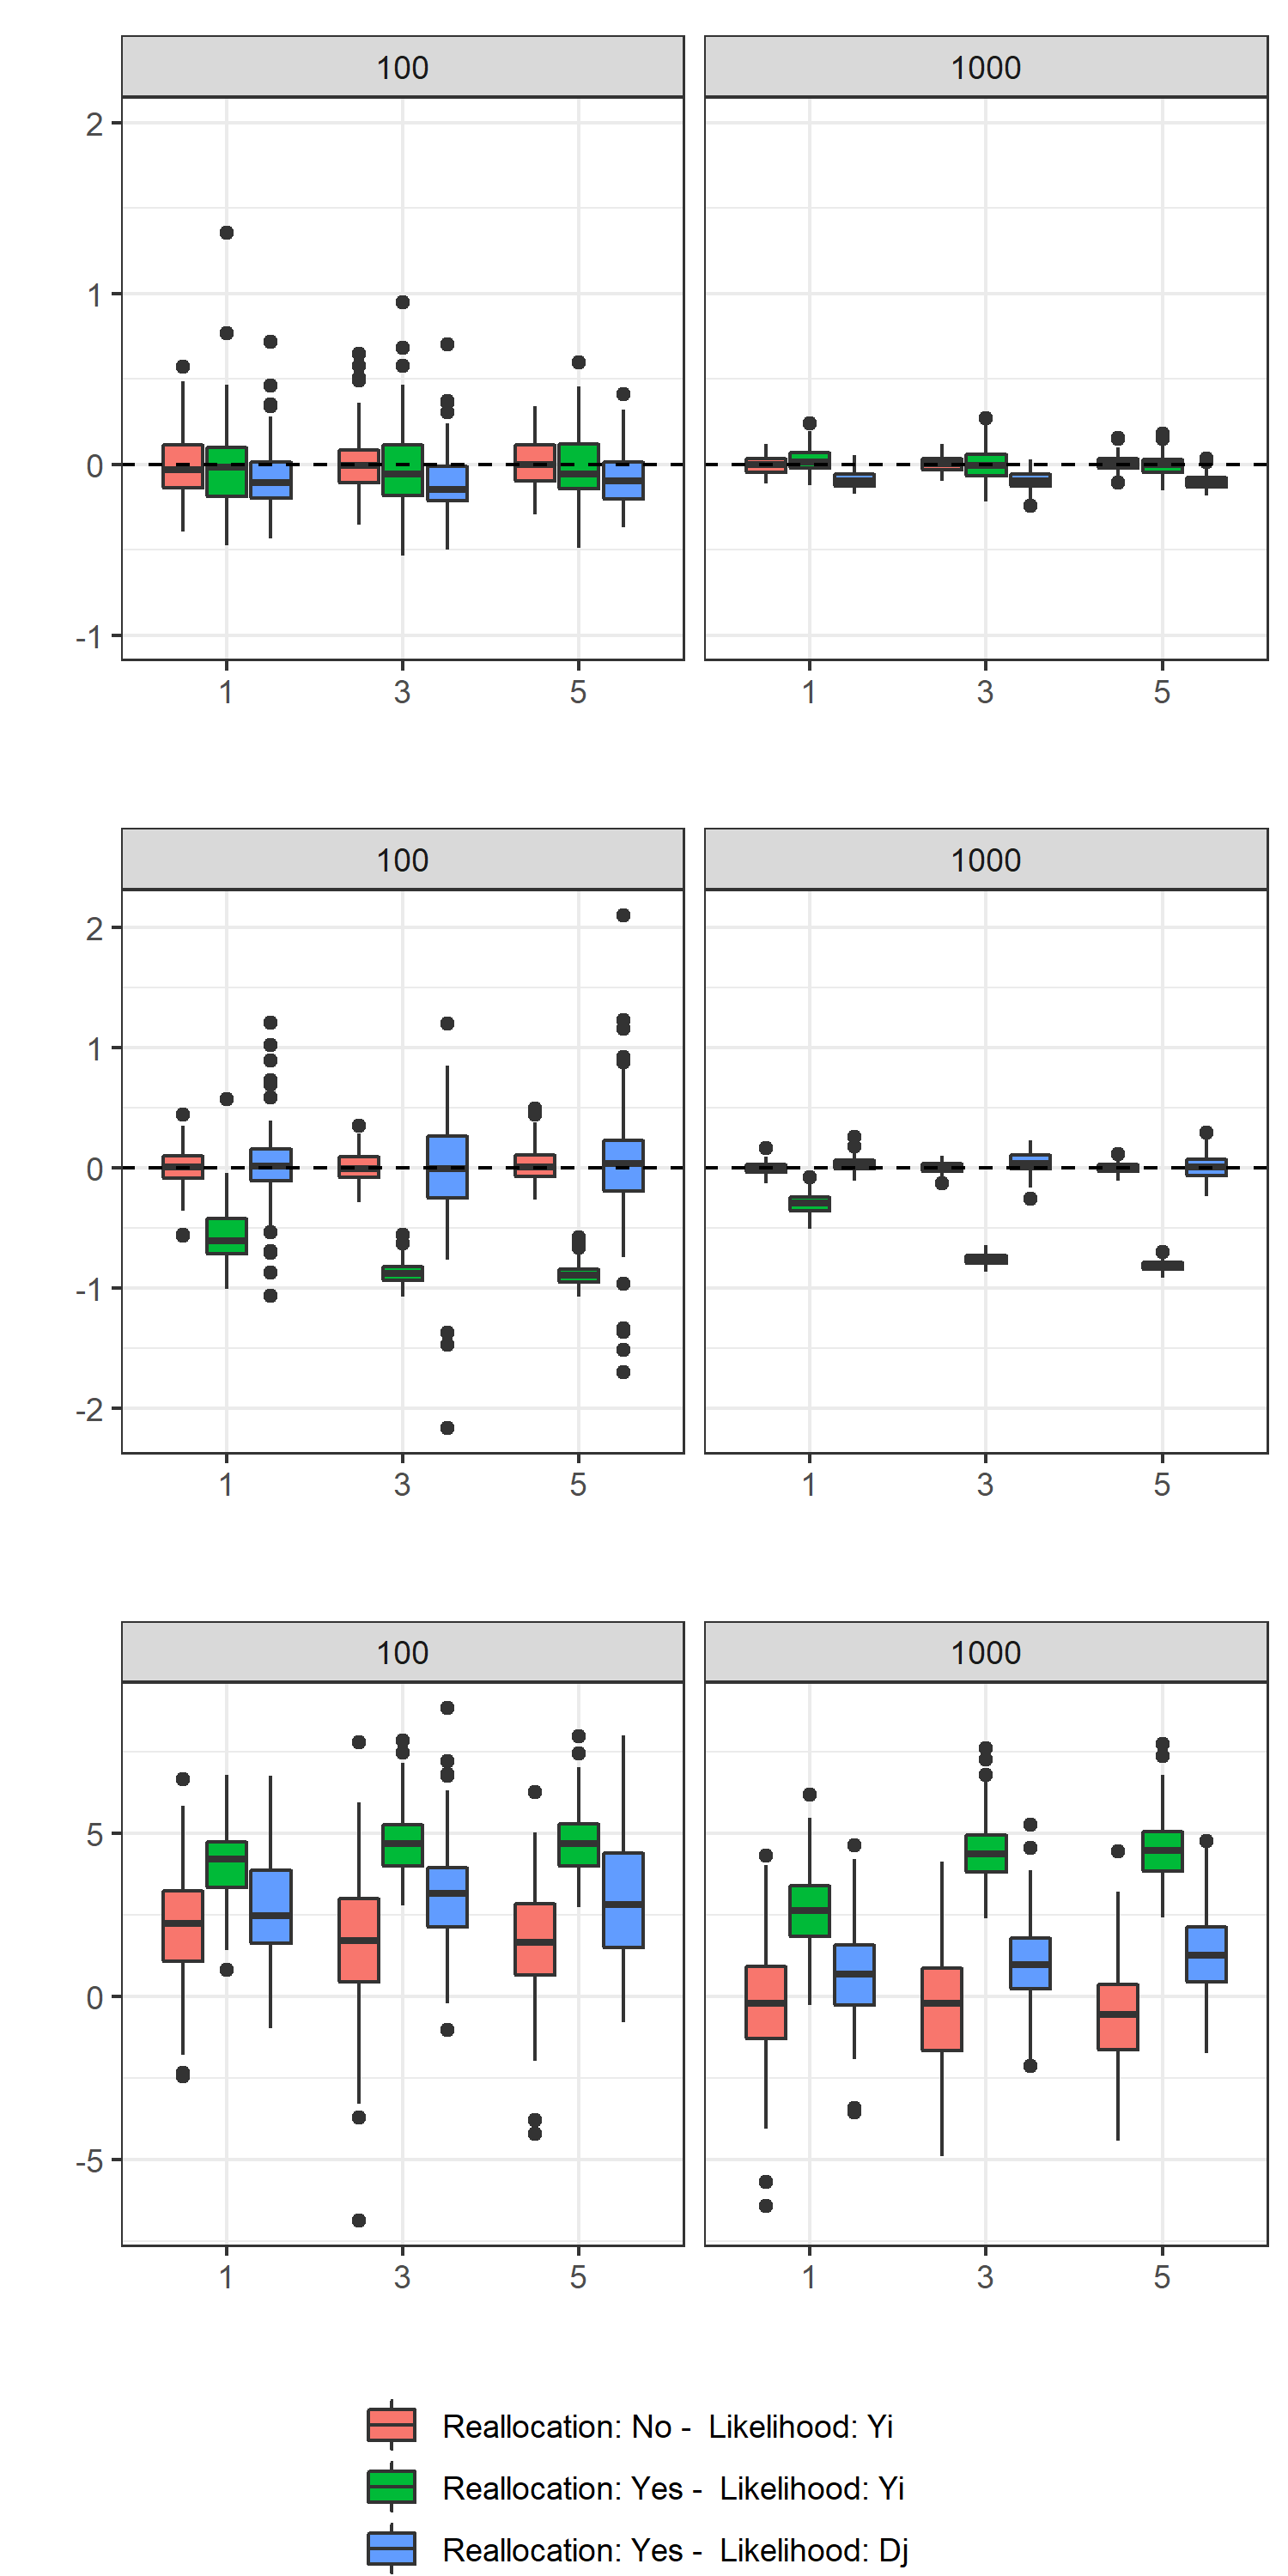
\includegraphics{images/Perf.metric_single_square.png}
\caption{\label{fig:PerfMetricSingle} Performance metric for single-square simulations. columns: number of commercial pings. x-axis: number of zones visited within each declaration. \enquote{Reallocation:}, data are or are not reallocated in simulations. \enquote{Likelihood:}, the likelihood is computed on reallocated observations \(Y_i\) or on catch declarations \(D_j\). Gold: golden standard. Gold: golden standard. Red: uniform reallocation situation. Green: model-based reallocation (declaration-based model). Simulations conducted on 10 fishing positions are not represented as they mostly did not converged for the declaration-based model.}
\end{figure}

Reallocation has a major effect on predictions and estimates accuracy (Figure \ref{fig:PerfMetricSingle}). Reallocating data conduct to a 10 to 200 times decrease of predictions accuracy when working at punctual observations (\(Y_i\)) level (MSPE gold compared to red boxplots). Accuracy decreases as the number of visited zones within a declaration increases. It also leads to the loss of the species-habitat relationship as the \(\beta_S\) estimates are biased; furthermore, estimates tend towards 0 as the number of fishing zones within a declaration increases. Increasing the number of samples does not improve inference. Regarding other parameters estimates (\(\mu\),\(\xi\),\(\sigma\)), the zero-inflation parameter (\(\xi\)) is over-estimated (i.e.~when uniformly reallocating commercial data, the quantity of positive observations is under-estimated), the observation variance (\(\sigma\)) is underestimated (i.e.~the data is estimated to be less noisy than they actually are) and the intercept of the latent field (\(\mu\)) is slightly over-estimated (Figure \ref{fig:ParBiasSingle}).

The declaration-based model (\(D_j\)) allows to recover the species-habitat relationship and to improve the accuracy of the spatial predictions (Figure \ref{fig:PerfMetricSingle}). Still, the declaration-based model outputs are not as accurate as the ones of the golden-standard. Furthermore, the zero-inflation parameter is unbiased when the likelihood is built on catch declarations \(D_j\). Other parameters (observation variance, intercept) are also better estimated even though they remain slightly biased (Figure \ref{fig:ParBiasSingle}). This alternative model have some convergence difficulties (Table 1) as 8\% of the model did not converged when sample size is medium (100 pings) and only 3\% did not when sample size is large (1000 pings).

\begin{figure}
\centering
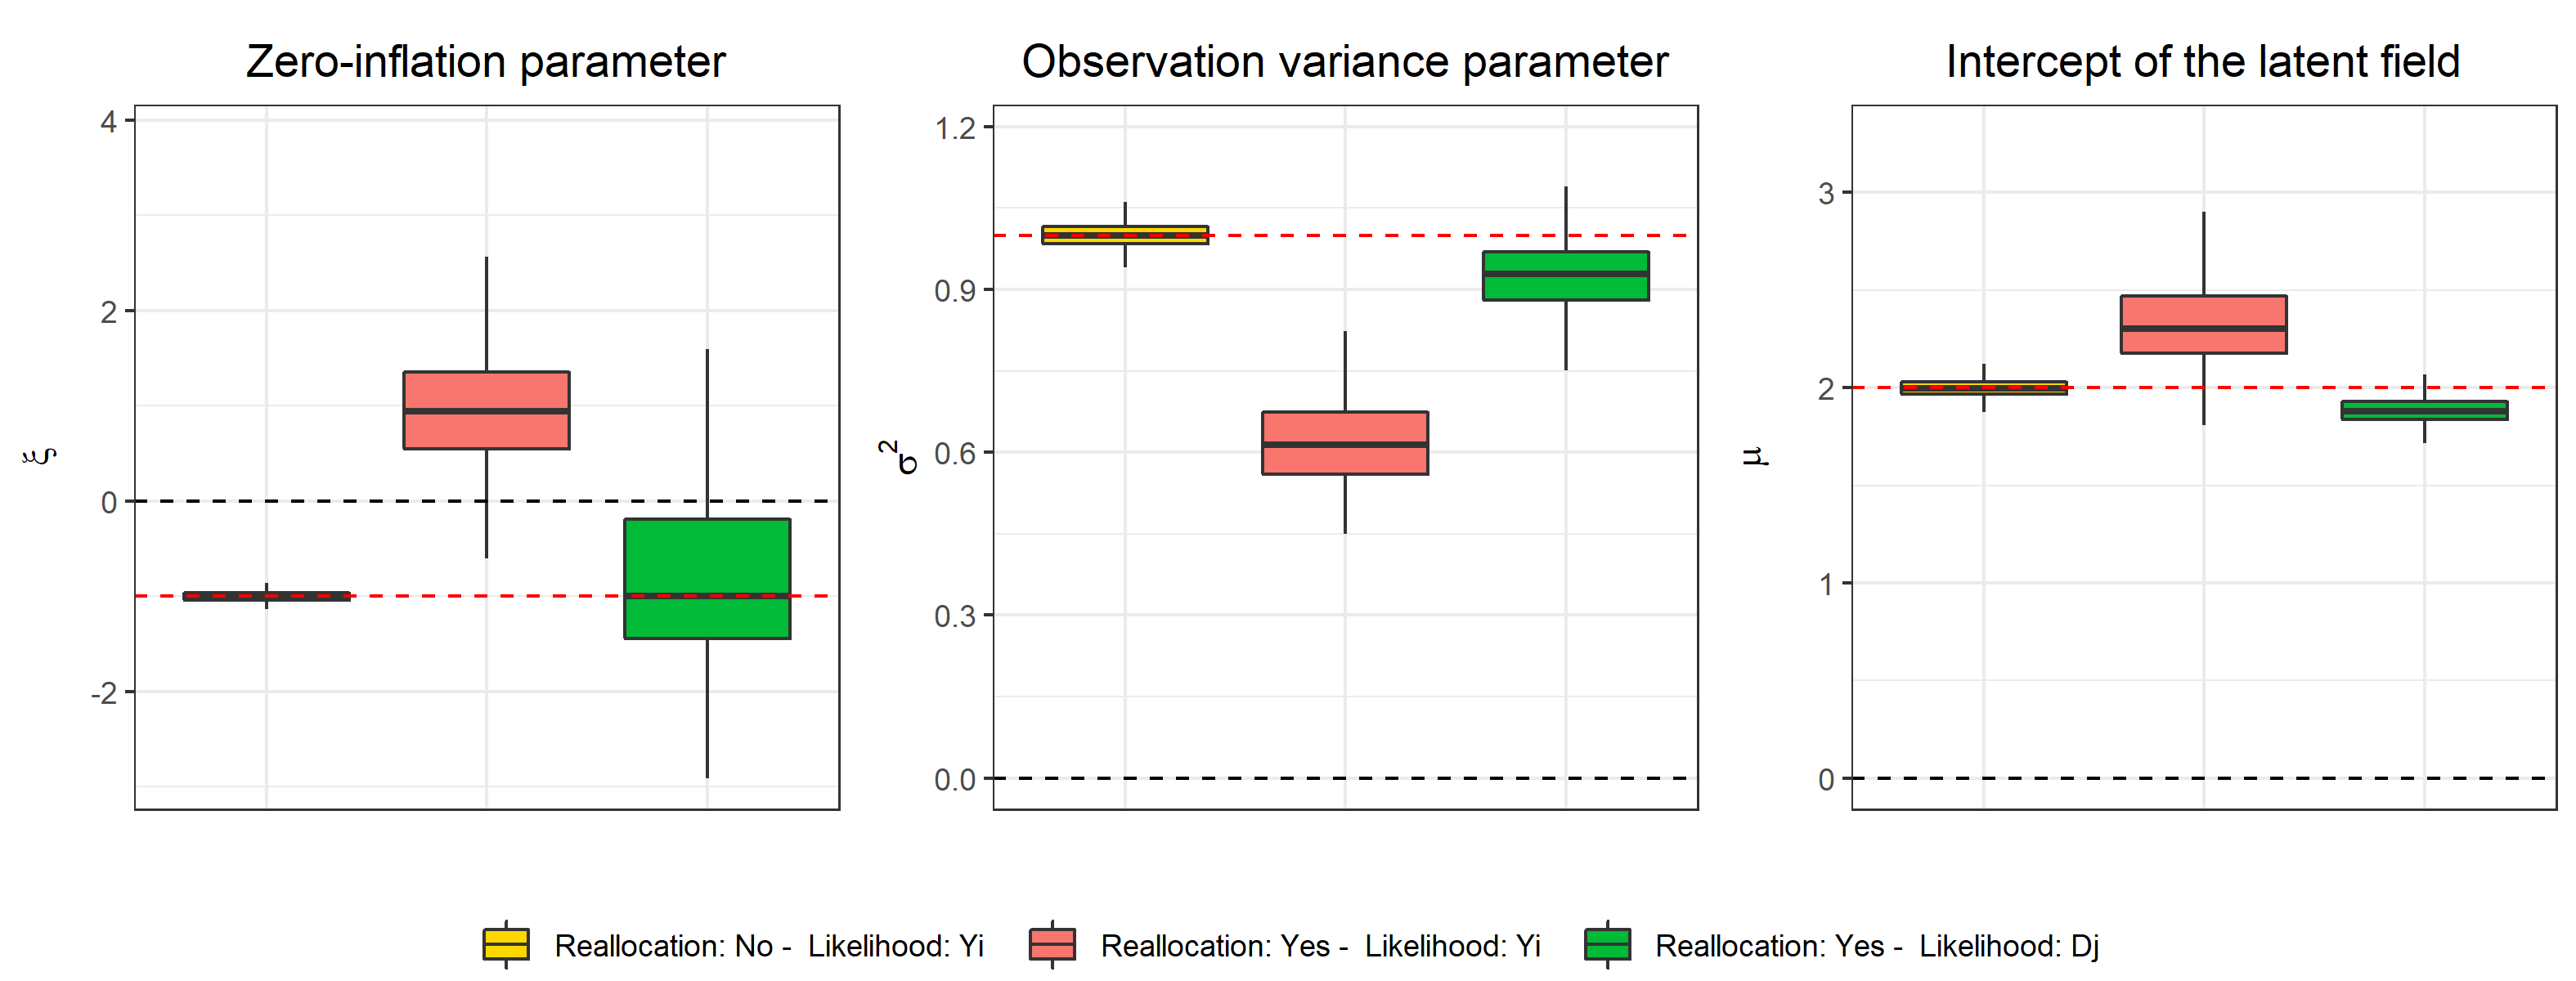
\includegraphics{images/par_plot_single_square.png}
\caption{\label{fig:ParBiasSingle} Parameters relative bias for single-square simulations. \enquote{Reallocation:}, data are or are not reallocated in simulations. \enquote{Likelihood:}, the likelihood is computed on reallocated observations \(Y_i\) or on catch declarations \(D_j\). Gold: golden standard. Red: uniform reallocation situation. Green: model-based reallocation (declaration-based model). Only the simulations with 1000 fishing positionss are represented. Black line: zero value. Red line: parameter true value.}
\end{figure}

\hypertarget{multiple-square-analysis}{%
\subsection{Multiple square analysis}\label{multiple-square-analysis}}

\begin{table}

\caption{\label{tab:unnamed-chunk-4}Percentage of convergence per simulation/model configuration at the level of several ICES rectangles}
\centering
\begin{tabular}[t]{ccc}
\toprule
Model & Likelihood level & Convergence (\%)\\
\midrule
Commercial model & Yi & 100.000\\
Commercial model & Dj & 75.377\\
Integrated model & Yi & 100.000\\
Integrated model & Dj & 76.382\\
Scientific model &  & 100.000\\
\bottomrule
\end{tabular}
\end{table}

\begin{verbatim}
## Warning: Removed 7 rows containing non-finite values (stat_boxplot).
\end{verbatim}

The scientific-based model provides species-habitat relationship and range estimates that are unbiased. Whether the model is built on \(Y_i\) or on \(D_j\), the contribution of either scientific or commercial data can be clearly evidenced from the MSPE plot: the errors related to the integrated model are smaller than the single-data models. This can be well evidenced when looking at Figure \ref{fig:MapSeveral}. Integrating scientific and commercial data allows to (1) capture the hotspot missed by commercial data through scientific data and (2) better capture the local correlation structures through the dense commercial data.

Furthermore, consistently with single-square simulations, uniform reallocation conducts to a loss in both the predictions accuracy and the species-habitat relationship (Figure \ref{fig:PerfMetricSeveral}) compared to the model built on commercial declarations (\(D_j\)).

Interestingly, uniform reallocation does not affect only the species-habitat relationship but also the spatial autocorrelation terms such as the range parameter. The model fitted on reallocated data (\(Y_i^*\)) provides biased range estimates while the declaration-based model provides unbiased estimates. This is a consequence of the loss of the species-habitat relationship: when uniformly reallocating declarations, part of the variability related to the covariate effect is captured by the random effect and then the range parameter captures both autocorrelation related to the actual random effect and to the covariate.

Working the declaration-based model allows to recover and disentangle the effect of the species-habitat relationship and of the random effect. This is evidenced in Figure \ref{fig:MapSeveral} where the model based on reallocated catch \(Y_i^*\) provides smoothed maps and do not captures the relatively small scale patterns that are shaped by the covariate effect. On the other hand the declaration-based model (and the scientific-based model too) better capture and disentangle the covariate effect and the spatial random effect and then provide predictions that better fit to the small-scale patterns of the species distribution. However, this goes with some difficulty in convergence as only 75\% of the model built on catch declarations converge (Table 2).

\begin{figure}
\centering
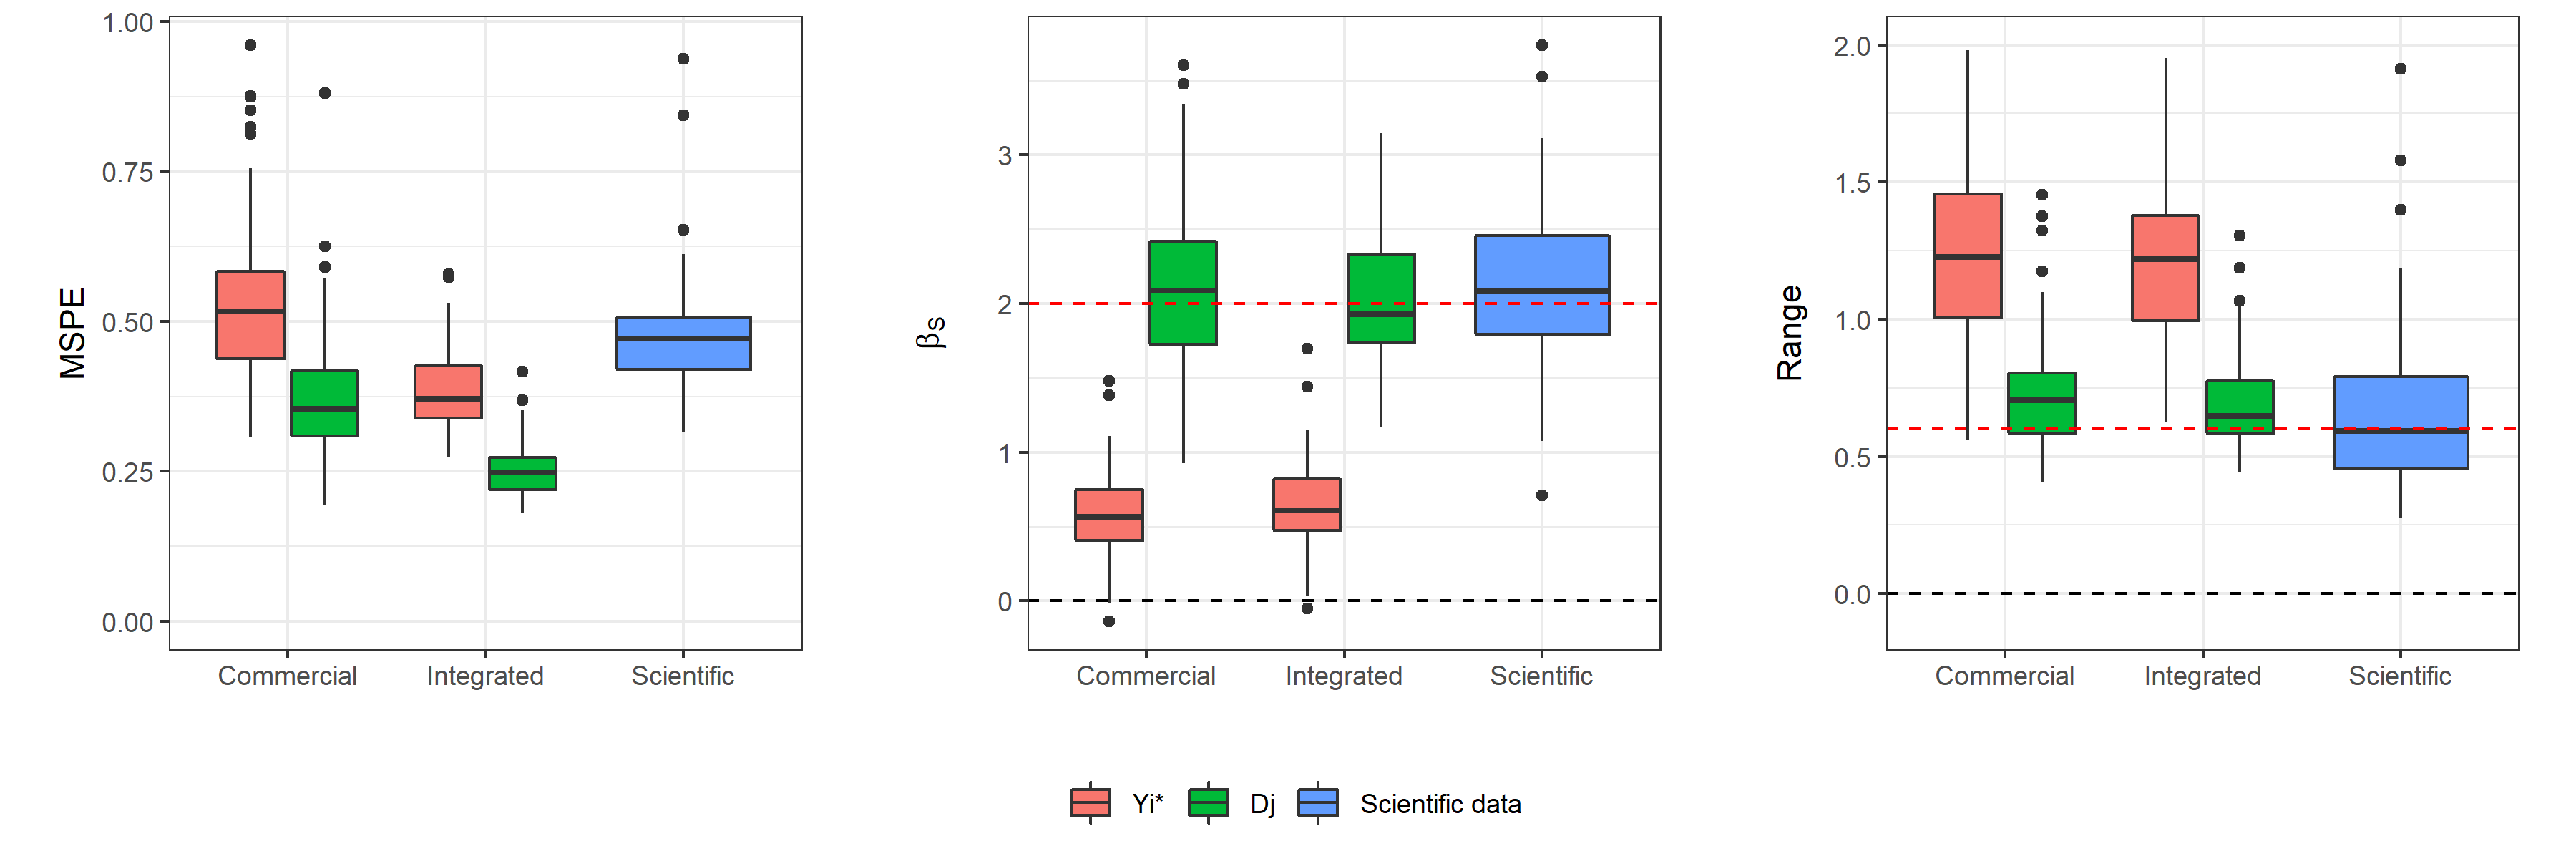
\includegraphics{images/Perf.metric_multiple_square.png}
\caption{\label{fig:PerfMetricSeveral} Performance metric for several rectangles simulations. columns: commercial data coverage. x-axis: likelihood level. \(1^{st}\) row, red line: true value of \(\beta_S\).}
\end{figure}

\begin{figure}
\centering
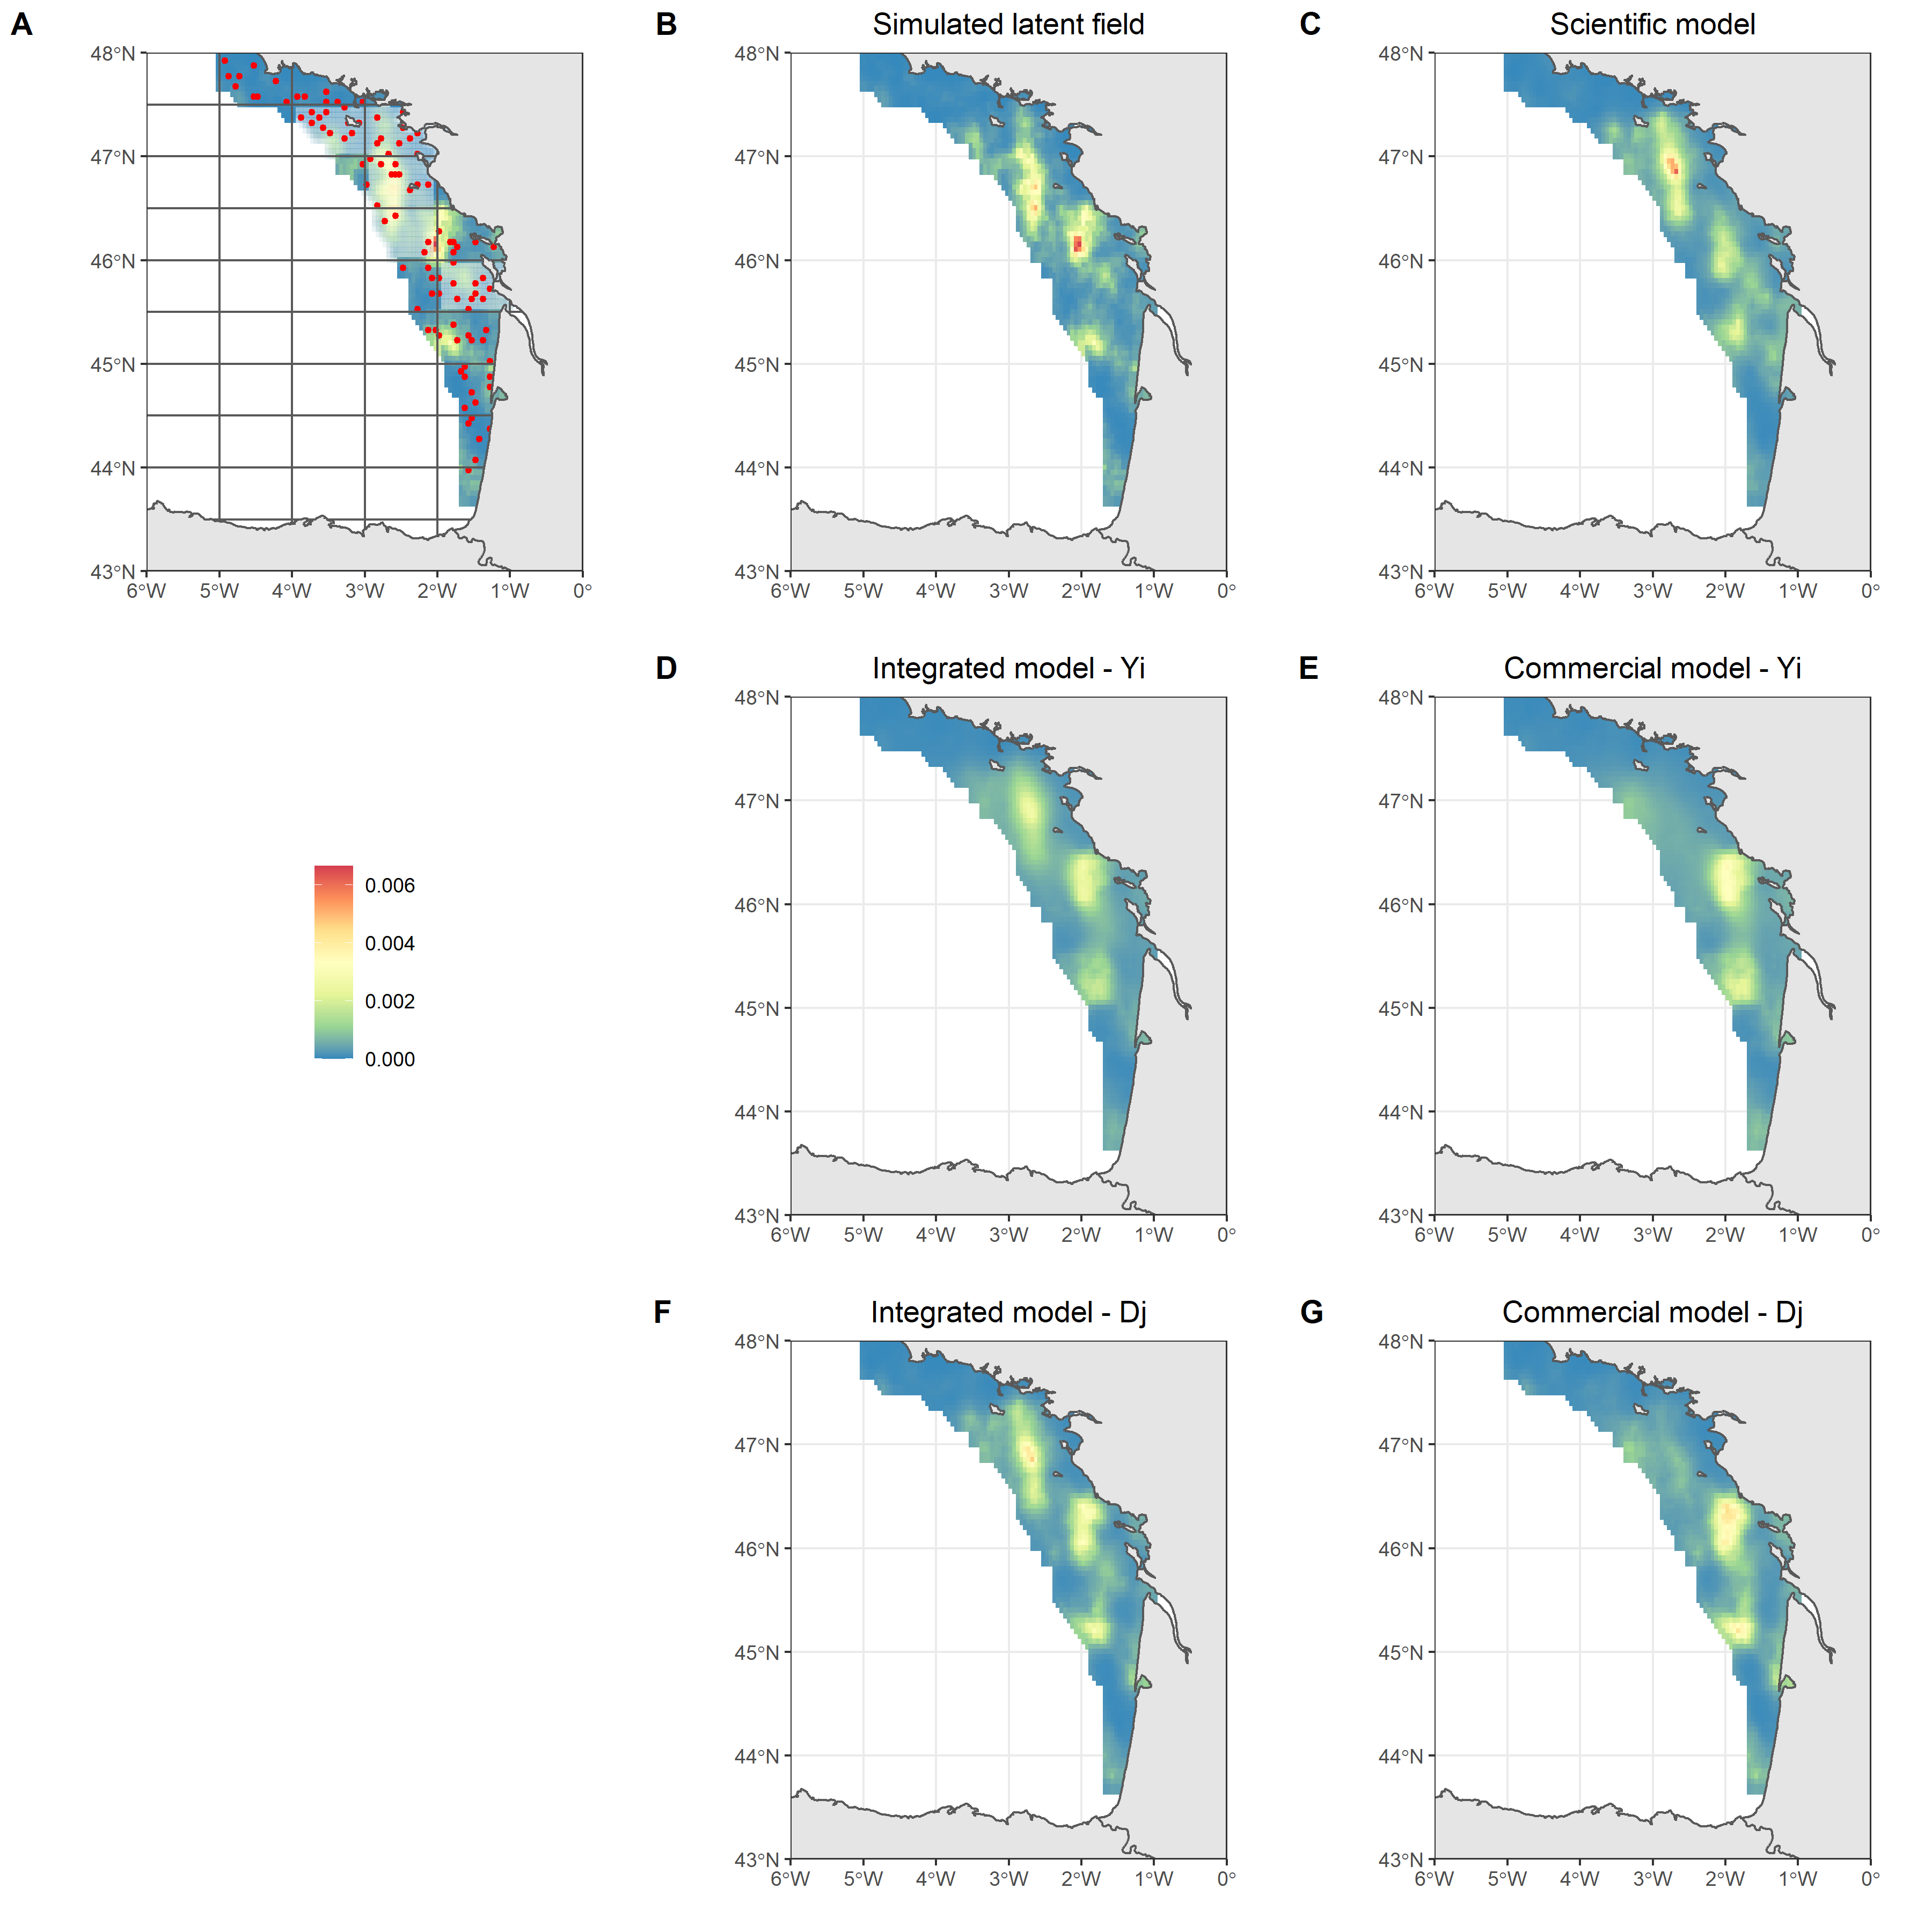
\includegraphics{images/Map_multi_square.png}
\caption{\label{fig:MapSeveral} Relative distribution of simulated/estimated biomass field. A: Simulated biomass field with scientific samples (red) and rectangles that have not been sampled by commercial data (transparent rectangles). B: simulated biomass field. C: biomass field from the scientific-based model. \(Y_i\): model fitted at the punctual observation level (D, E). \(D_j\): declaration-based model (F, G).}
\end{figure}

\hypertarget{real-case-study}{%
\subsection{Real case study}\label{real-case-study}}

\begin{figure}
\centering
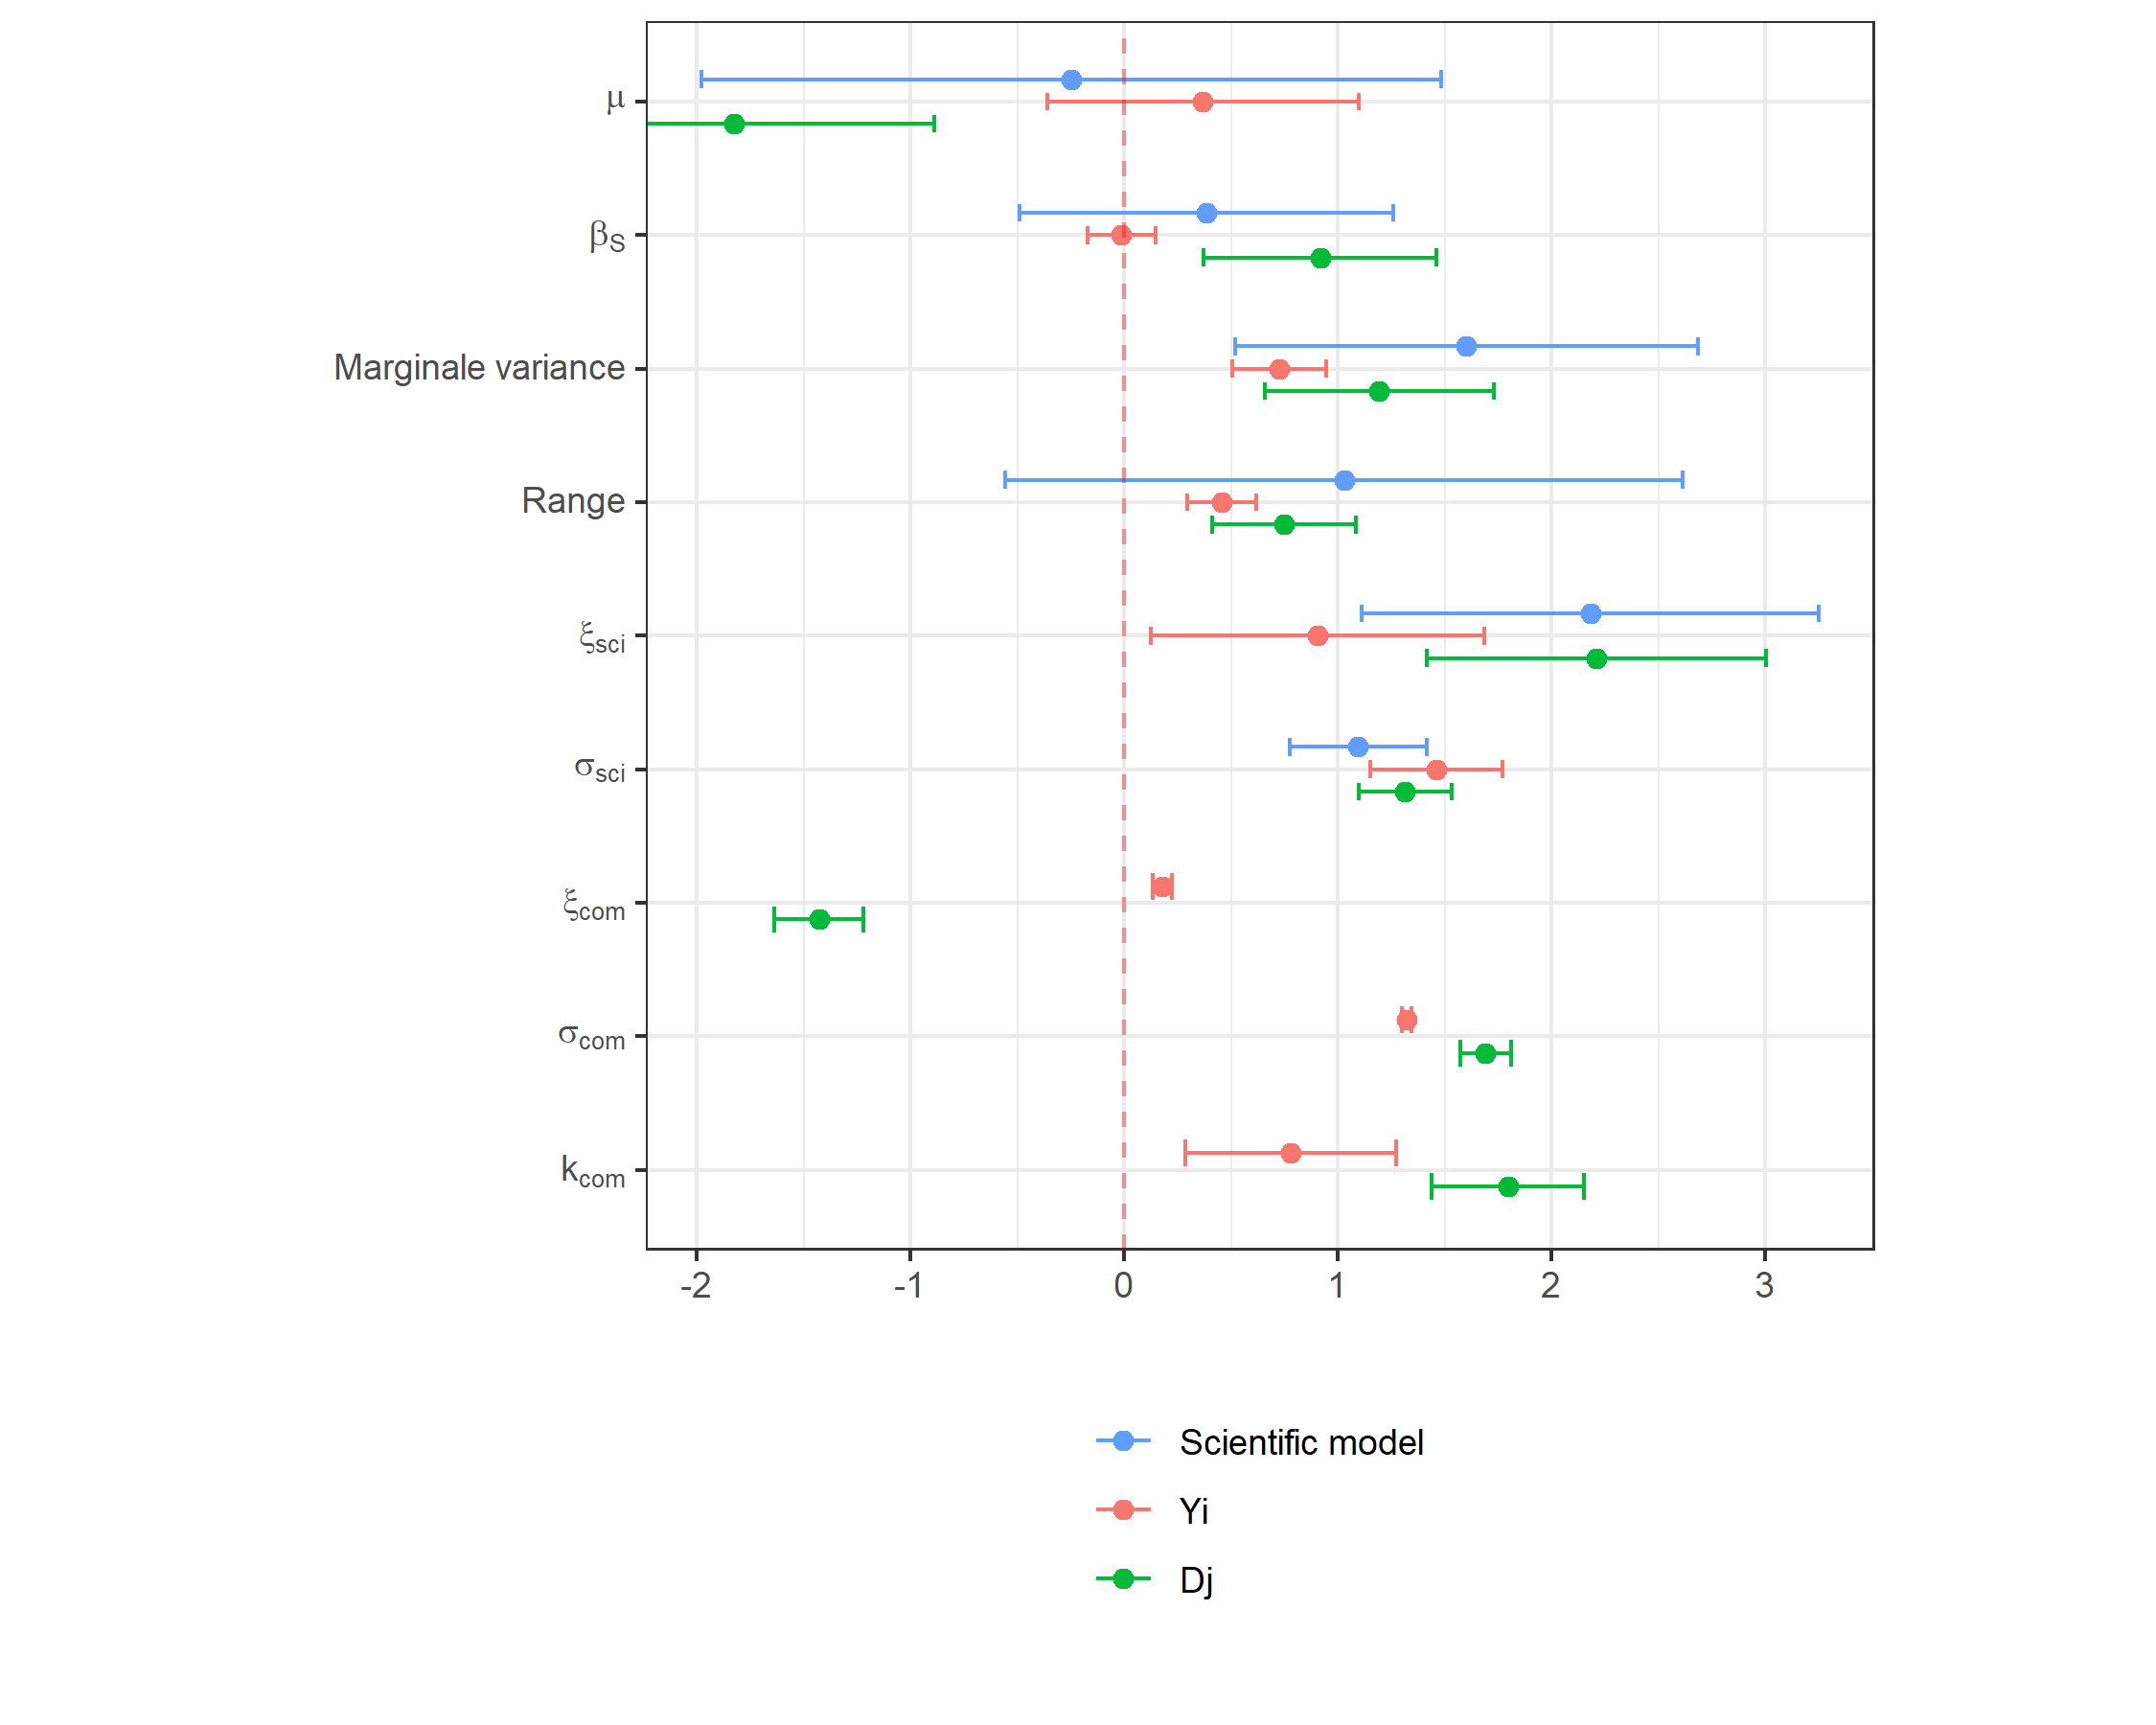
\includegraphics{images/par_plot.png}
\caption{\label{fig:CaseStudyPar} Parameters obtained with scientific-based model, the integrated model fitted on reallocated catch \(Y_i^*\) and the integrated model fitted on catch declarations \(D_j\).}
\end{figure}

\begin{figure}
\centering
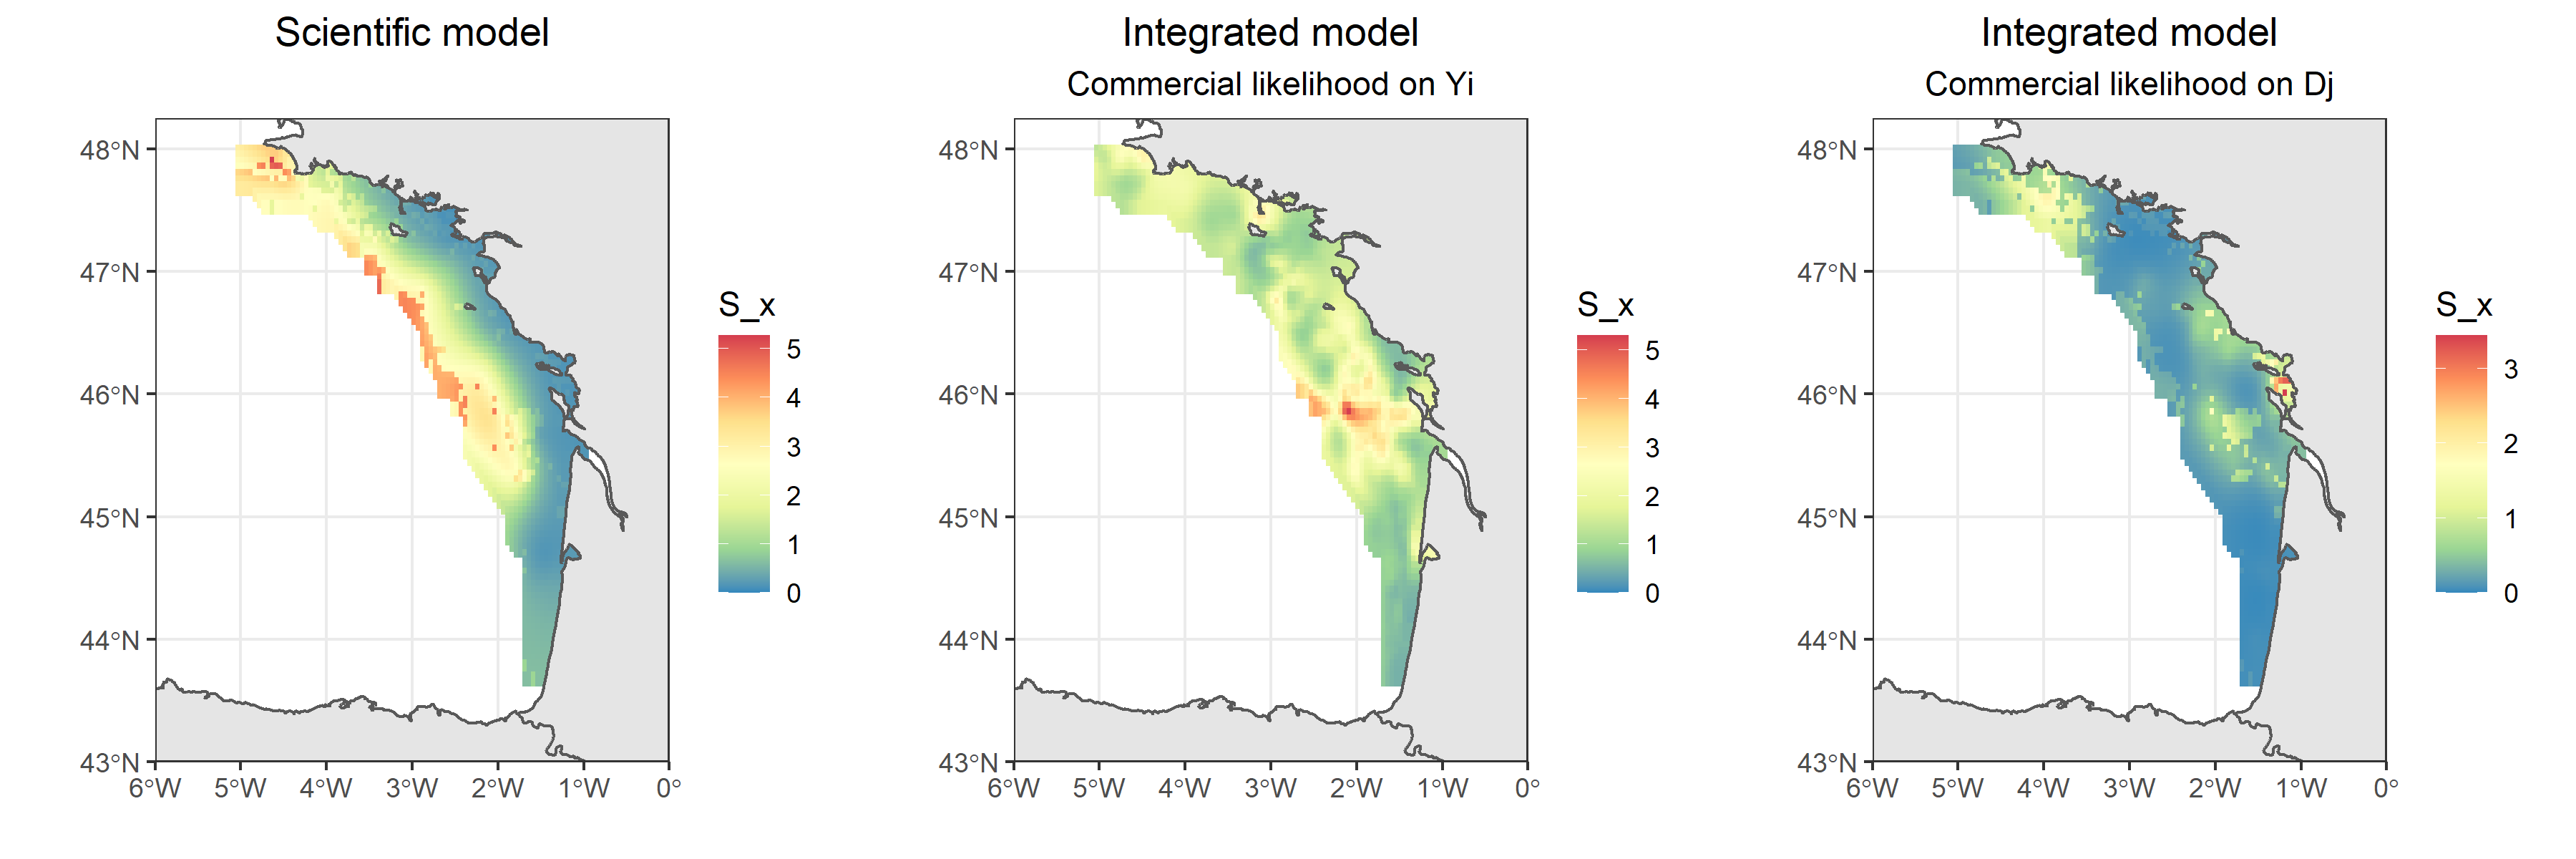
\includegraphics{images/case_study_plot.png}
\caption{\label{fig:CaseStudyMap} Maps obtained from (left) the scientific-based model, (center) the integrated model fitted on punctual observations \(Y_i^*\), (right) the integrated model fitted on catch declarations \(D_j\).}
\end{figure}

Passing from punctual observations \(Y_i^*\) to catch declarations \(D_j\) modifies the overall distribution patterns. Besides, some of the parameters estimates are modified consistently with simulations. The model fitted on \(Y_i^*\) tend to provide biased estimates and under-estimate the uncertainty related to other estimates compared with the scientific-based model and the declaration-based model. In particular, the substrate effect is recovered in both models (Figure \ref{fig:CaseStudyMap}). The zero-inflation parameter \(\xi\) is revised downwards (i.e.~there are actually more zero-values than in the reallocated data) while the observation variance of commercial data is revised upwards (i.e.~the commercial data are more noisy than expected when building likelihood on \(Y_i\)). In addition, related confidence intervals (CI) are also revised when fitting the model at the declaration level. Specifically, the CI from \(\beta_S\), the marginal variance, the range, \(\xi_{com}\), \(\sigma_{com}\) are very narrow in the model fitted to reallocated catch while in the model fitted to \(D_j\) confidence intervals are larger. This emphasizes that uncertainty is probably underestimated in the model fitted to reallocated catch compared with the declaration-based model.

Now, when comparing the scientific-based model and the integrated model fitted on \(D_j\), some parameters are better estimated. For instance, while in the scientific-based model the substrate effect was not significant, in the integrated model built on \(D_j\) substrate is significant and the confidence interval is smaller. Other parameters are more precisely estimated such as the marginal variance, the range, \(\xi_{sci}\) and \(\sigma_{sci}\).

On the contrary, other parameters do not seems be well estimated in either the \(Y_i^*\) or the \(D_j\) models. For instance, compared to the scientific-based model, the intercept is revised upwards when building the likelihood on \(Y_i\) and revised downards when working on \(D_j\). This is consistent with simulations results, see Figure \ref{fig:ParBiasSingle}.

Regarding the maps of the spatial predictions, fitting the model at the \(D_j\) level strongly modifies the model biomass field compared with the \(Y_i^*\) model. In particular, the effect of the covariate have a sharper effect on species distribution. Furthermore, the intensity of the hotspots are revised when fitting the model on \(D_j\).

Finally, the \(D_j\) model fitted only on commercial data does not converge (while the one built on \(Y_i\) does) emphasizing the model build on catch declarations face difficulties to converge and require punctual observations (here survey data and on-board observer data) to converge on real data.

\hypertarget{discussion}{%
\section{Discussion}\label{discussion}}

\newpage

\hypertarget{references}{%
\section{References}\label{references}}

\begingroup
\setlength{\parindent}{-0.5in}
\setlength{\leftskip}{0.5in}

\hypertarget{refs}{}
\leavevmode\hypertarget{ref-alglave_combining_2022}{}%
Alglave, B., Rivot, E., Etienne, M.-P., Woillez, M., Thorson, J. T., \& Vermard, Y. (2022). Combining scientific survey and commercial catch data to map fish distribution. \emph{ICES Journal of Marine Science}, fsac032. \url{https://doi.org/10.1093/icesjms/fsac032}

\leavevmode\hypertarget{ref-biais_gerard_orhago_2003}{}%
Gérard, B. (2003). ORHAGO. \url{https://doi.org/10.18142/23}

\leavevmode\hypertarget{ref-ices_report_2018-1}{}%
ICES. (2018a). \emph{Report of the Working Group for the Bay of Biscay and the Iberian Waters Ecoregion (WGBIE)} (p. 642). Copenhagen, Denmark.

\leavevmode\hypertarget{ref-ices_report_2018}{}%
ICES. (2018b). \emph{Report of the Working Group on Beam Trawl Surveys (WGBEAM)} (p. 121). Galway, Ireland.

\leavevmode\hypertarget{ref-kristensen_tmb_2016}{}%
Kristensen, K., Nielsen, A., Berg, C. W., Skaug, H., \& Bell, B. M. (2016). TMB: Automatic Differentiation and Laplace Approximation. \emph{Journal of Statistical Software}, \emph{70}(1), 1--21. \url{https://doi.org/10.18637/jss.v070.i05}

\leavevmode\hypertarget{ref-thorson_three_2018}{}%
Thorson, J. T. (2018). Three problems with the conventional delta-model for biomass sampling data, and a computationally efficient alternative. \emph{Canadian Journal of Fisheries and Aquatic Sciences}, \emph{75}(9), 1369--1382.

\endgroup


\end{document}
